\documentclass[11pt,twocolumn]{article}
\usepackage[a4paper,margin=2.2cm]{geometry}
\usepackage[T1]{fontenc}
\usepackage{lmodern}
\usepackage{graphicx}
\usepackage{xcolor}
\usepackage{needspace}
\usepackage{tikz}
\newcommand{\cartoon}[2]{\begin{figure}[!htb]\centering #1\par\smallskip\noindent\begin{minipage}{\columnwidth}\small\sffamily #2\end{minipage}\end{figure}}
\usepackage{microtype}
\setlength{\columnsep}{0.8cm}
\setlength{\parindent}{1.2em}
\setlength{\parskip}{0pt}
\definecolor{accent}{RGB}{150,30,30}
\newcommand{\sect}[1]{\par\needspace{5\baselineskip}\medskip{\sffamily\bfseries\color{accent}\MakeUppercase{#1}}\par\smallskip\noindent}
\pagestyle{plain}

\begin{document}

\twocolumn[{\begin{center}
{\sffamily\small\color{accent}MATERIALS SCIENCE}\\[6pt]
{\sffamily\bfseries\LARGE Order Is Not Destiny}\\[8pt]
{\large\itshape Two materials built from the same pattern can differ in how\\ they carry a load. The difference lies in whether their struts line up}\\[10pt]
{\sffamily\small A summary of ``Classes of metamaterials generated by recursive cell division'' by Alexei Vazquez}
\end{center}\vspace{10pt}}]

\noindent{\sffamily\bfseries\large P}ick up a sheet of corrugated cardboard and squeeze it along the ribs: it resists. Squeeze it across them and it gives. The cardboard is the same material in both directions. What changes is the path the force has to follow. Engineers who design \emph{metamaterials}---solids whose behaviour comes from their architecture more than from their chemistry---live by this lesson. A lattice of thin struts can be as stiff as a bridge truss or as soft as a sponge, depending only on how the struts are arranged.

For decades the arrangement has been described with one word: \emph{order}. Crystals are periodic, with a pattern that repeats like wallpaper. Quasicrystals, whose discovery earned Dan Shechtman the 2011 Nobel Prize in Chemistry, are ordered without repeating, like the famous Penrose tilings. Glasses and foams are disordered. A tacit assumption runs through much of the field: the more ordered a framework, the more its struts line up into the long straight beams that make it stiff.

The new work asks whether that assumption holds. Its answer is no. Order and alignment turn out to be two separate properties of a framework, and they can be dialled independently.

\sect{Why straight lines matter}
Picture a window grid of horizontal and vertical bars. Pull it sideways and each horizontal bar that runs from one edge to the other must stretch. Stretching a bar is hard, so the grid is stiff. Now break those long bars into short pieces whose ends are staggered, like the bricks in a wall. Pull the same way and the pieces have no continuous path to stretch along; the frame yields instead by bending its joints. Bending is easy, so the frame is soft.

\cartoon{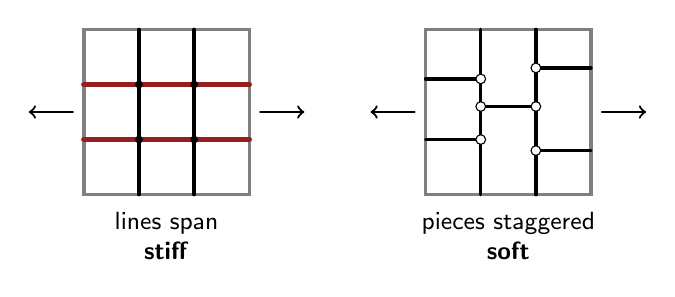
\begin{tikzpicture}[scale=0.7,line cap=round]
\begin{scope}
\draw[gray,line width=1.2pt] (0,0) rectangle (3,3);
\foreach \x in {1,2} \draw[line width=1.2pt] (\x,0)--(\x,3);
\foreach \y in {1,2} \draw[accent,line width=2pt] (0,\y)--(3,\y);
\foreach \x in {1,2} \foreach \y in {1,2} \fill (\x,\y) circle (2pt);
\draw[->,thick] (-0.2,1.5)--(-1,1.5); \draw[->,thick] (3.2,1.5)--(4,1.5);
\node[font=\sffamily\small,align=center] at (1.5,-0.75) {lines span\\\textbf{stiff}};
\end{scope}
\begin{scope}[xshift=6.2cm]
\draw[gray,line width=1.2pt] (0,0) rectangle (3,3);
\foreach \x in {1,2} \draw[line width=1.2pt] (\x,0)--(\x,3);
\draw[line width=1.2pt] (0,1.0)--(1,1.0) (0,2.1)--(1,2.1) (1,1.6)--(2,1.6) (2,0.8)--(3,0.8) (2,2.3)--(3,2.3);
\foreach \p in {(1,1.0),(1,2.1),(1,1.6),(2,1.6),(2,0.8),(2,2.3)} \filldraw[fill=white,draw=black] \p circle (2.5pt);
\draw[->,thick] (-0.2,1.5)--(-1,1.5); \draw[->,thick] (3.2,1.5)--(4,1.5);
\node[font=\sffamily\small,align=center] at (1.5,-0.75) {pieces staggered\\\textbf{soft}};
\end{scope}
\end{tikzpicture}}{\textbf{Why straight lines matter.} Pulled sideways, a grid whose bars cross the whole frame (left, red) must stretch them. When the bars are broken into staggered pieces (right), no bar crosses; the frame gives by bending at its joints (circles). Turn those joints into free hinges and the right frame offers no resistance, apart from its outer border.}

Materials scientists call the first kind \emph{stretch dominated} and the second \emph{bending dominated}. A simple test tells them apart: replace every welded joint with a free hinge. A stretch-dominated frame stays stiff. A bending-dominated frame collapses, because its stiffness lived in the joints.

The paper turns this test into an exact counting rule. For a frame of horizontal and vertical bars with hinged joints, the stiffness in a given direction equals the number of straight lines that cross the whole sample in that direction, times the stiffness of a single bar. Nothing else counts---not how many bars there are, not how short or long they are. A line that stops short of the edge simply slides along at no cost. The count of spanning lines is the stiffness.

\sect{Growing a material by cutting}
To study order and alignment together, the paper grows frameworks with one simple procedure. Start with a square. Cut it in two. Then take the largest piece and cut it across its long side. Repeat, thousands or millions of times. Each cut becomes a strut, and the result is a tiling of rectangles (see figure).

The rule for each cut has two parts. The first is \emph{where} along the piece to cut, written as a fraction $r_0$ of its length. Cut every piece in half and you get an ordinary checkerboard grid. Cut every piece at the golden ratio and you get a quasicrystal. Cut each piece at a random point and you get disorder.

\begin{figure*}[t]
\centering
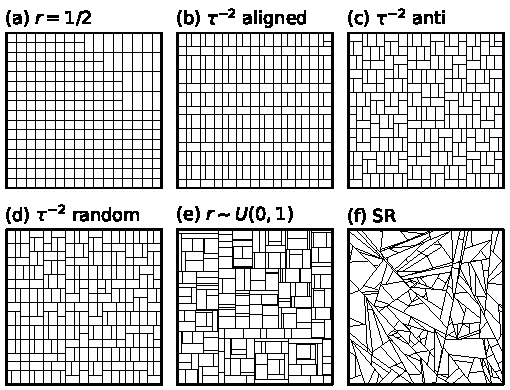
\includegraphics[width=0.82\textwidth]{fig1.pdf}
\par\smallskip
\begin{minipage}{0.88\textwidth}\small\sffamily
\textbf{Same recipe, different architectures.} Each panel is a square cut 233 times by the rule described in the text. (a) Cutting every piece in half gives an ordinary grid. (b)--(d) Cutting at the golden ratio gives a quasicrystal; what differs is the end of each piece from which the cut is measured. Measured always from the same end (b), the cuts line up into long straight lines across the square. Measured from the end that avoids lining up (c), only the first cut crosses the whole square. Chosen by a coin toss (d), the result lies in between. (e) Cutting at random points gives a disordered tiling. (f) A ``scale-rich'' design, with random cuts at random angles.
\end{minipage}
\end{figure*}

The second part of the rule is easy to overlook: \emph{from which end} of the piece the fraction is measured. Cutting a strip one third of the way along from the left is not the same as cutting it one third of the way from the right. The paper compares three choices: always from the same end (the \emph{aligned} rule), the end chosen by a coin toss (\emph{random}), and the end that avoids continuing a cut already made on the other side of the strut (\emph{anti-aligned}).

\cartoon{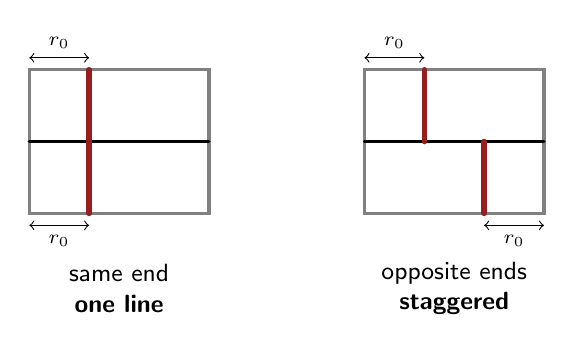
\begin{tikzpicture}[scale=0.76,line cap=round]
\foreach \sh/\lo/\lab in {0/1/{same end\\\textbf{one line}},5.6/2/{opposite ends\\\textbf{staggered}}}{
\begin{scope}[xshift=\sh cm]
\draw[gray,line width=1.2pt] (0,0) rectangle (3,2.4);
\draw[line width=1.2pt] (0,1.2)--(3,1.2);
\ifnum\lo=1 \draw[accent,line width=2pt] (1,0)--(1,2.4);
\else \draw[accent,line width=2pt] (1,1.2)--(1,2.4); \draw[accent,line width=2pt] (2,0)--(2,1.2); \fi
\draw[<->,thin] (0,2.6)--(1,2.6) node[midway,above,font=\scriptsize] {$r_0$};
\ifnum\lo=1 \draw[<->,thin] (0,-0.2)--(1,-0.2) node[midway,below,font=\scriptsize] {$r_0$};
\else \draw[<->,thin] (3,-0.2)--(2,-0.2) node[midway,below,font=\scriptsize] {$r_0$}; \fi
\node[font=\sffamily\small,align=center] at (1.5,-1.25) {\lab};
\end{scope}}
\end{tikzpicture}}{\textbf{Which end?} Two pieces sit on either side of the same strut (black), and each is cut at the same fraction $r_0$ of its length. Measured from the same end (left), the two cuts meet and form one straight line. Measured from opposite ends (right), they miss each other.}

\sect{Two knobs, two properties}
The first knob, the cut fraction, decides the order. When the fraction is tied to a special family of numbers---the Pisot numbers, of which the golden ratio is the most famous---every junction in the tiling falls on a hidden lattice of positions. Shine a beam of waves through such a structure and it scatters into sharp, bright spots, the fingerprint of a quasicrystal. The paper shows this holds for each of the three end-choosing rules. Whichever end you measure from, the golden cut produces a quasicrystal.

The second knob, the end rule, decides the alignment. Under the aligned rule, every piece in a row is cut at the same height, so the cuts join into a perfect grid of straight lines spanning the sample; their number grows as the square root of the number of cuts. Under the anti-aligned rule, cuts are deliberately staggered. In all the simulations, up to a million cuts, only the very first cut ever runs from edge to edge.

So the same golden cut yields two quasicrystals with identical order and opposite architectures. One is threaded with straight lines; the other has almost none.

\sect{Stiff or soft}
The counting rule then predicts their mechanics. The aligned quasicrystal is stretch dominated: more than 90 percent of its stiffness survives when its joints are turned into hinges, at every size tested. The anti-aligned quasicrystal is bending dominated, and the share of its stiffness carried by stretching shrinks as the structure is refined, falling as one over the square root of the number of cuts. In a typical example of a light framework, stretching carries 94 percent of the load in the aligned version and 14 percent in the anti-aligned one.

In other words, the anti-aligned golden quasicrystal behaves mechanically like a random foam, while remaining as ordered as a Penrose tiling. It needs only three shapes of rectangle to build. This holds for slender frameworks, where the struts are thin compared with the gaps between them; in denser ones, nearly parallel struts merge into thick beams and the straight lines come back.

\sect{Beyond stiffness}
Waves also feel the difference, but not all waves feel the same thing. Some waves travel along a network of wires without caring about the angle at which wires meet---the electrons in a mesh of quantum wires, or the superconducting state in a grid of superconducting wires placed in a magnetic field. Their behaviour follows the order class alone, because bending a straight line into a crooked one only shifts their phase.

\cartoon{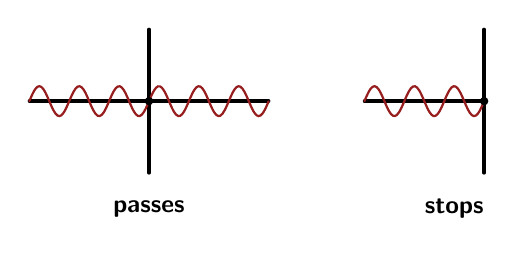
\begin{tikzpicture}[scale=0.76,line cap=round]
\begin{scope}
\draw[line width=1.2pt] (0,0)--(4,0); \draw[line width=1.2pt] (2,-1.2)--(2,1.2);
\draw[accent,thick,domain=0:4,samples=120,smooth] plot (\x,{0.25*sin(\x*540)});
\fill (2,0) circle (2pt);
\node[font=\sffamily\small,align=center] at (2,-1.8) {\textbf{passes}};
\end{scope}
\begin{scope}[xshift=5.6cm]
\draw[line width=1.2pt] (0,0)--(2,0); \draw[line width=1.2pt] (2,-1.2)--(2,1.2);
\draw[accent,thick,domain=0:2,samples=60,smooth] plot (\x,{0.25*sin(\x*540)});
\fill (2,0) circle (2pt);
\node[font=\sffamily\small,align=center] at (1.5,-1.8) {\textbf{stops}};
\end{scope}
\end{tikzpicture}}{\textbf{Spin waves follow straight lines.} The magnetism points along each wire. A spin wave ripples past a junction where its wire carries straight on (left), but is held back where its wire ends against another (right).}

Spin waves in a network of magnetic nanowires are different. The magnetism points along each wire, so a ripple in it passes smoothly through a junction only when the wire continues straight on. Here both knobs matter. In frameworks without straight lines the waves are trapped in small regions. In aligned frameworks they spread along the lines, and among those, only the ordered ones keep waves spread over a fixed share of the network as it grows.

\sect{Why should we care?}
The practical message is a gain in design freedom. A designer who wants a quasicrystalline pattern---for its sharp diffraction, its ability to steer certain waves, or its aesthetics---is not thereby committed to a stiff, brittle frame. The same pattern can be made stretch dominated or bending dominated by a choice that leaves the order untouched. Conversely, a designer who wants the compliance and damage tolerance of a foam can now ask for it in an ordered, reproducible architecture with a handful of building blocks, rather than in a random structure that varies from sample to sample.

The result also corrects a habit of thought. Order, measured by diffraction, records where the junctions sit. Alignment records which struts continue each other across a junction. The two come from different geometric features, and properties that depend on one need not depend on the other. A recently described class of \emph{scale-rich} metamaterials, grown by random cuts at random angles, was thought to owe its flexibility to its disorder. The present work shows that what it actually lacks is straight lines, and that an ordered framework can lack them too.

Some questions remain open. The claim that the anti-aligned rule never completes a second spanning line rests on simulations rather than proof. The analysis covers long-wavelength behaviour, not waves as short as a single cell. And all the cuts here are horizontal or vertical; allowing more directions, as in the pinwheel tilings, is the natural route to frameworks with rotational order. What is already clear is that, for a framework of struts, knowing its symmetry tells you only half the story. To know how it bears a load you also have to ask: where do its straight lines go?

\medskip
\noindent\rule{\linewidth}{0.4pt}\\
{\footnotesize\sffamily Based on A.\ Vazquez, \emph{Classes of metamaterials generated by recursive cell division}, Nodes \& Links Ltd, Cambridge (manuscript, 2026). Code: github.com/av2atgh/scalerich/tree/master/classes.}
\end{document}
